\chapter{Background}\label{chap:background}
\section{The Mass Balancing Problem}

\begin{figure}
    \centering
    \usetikzlibrary{arrows.meta,3d}
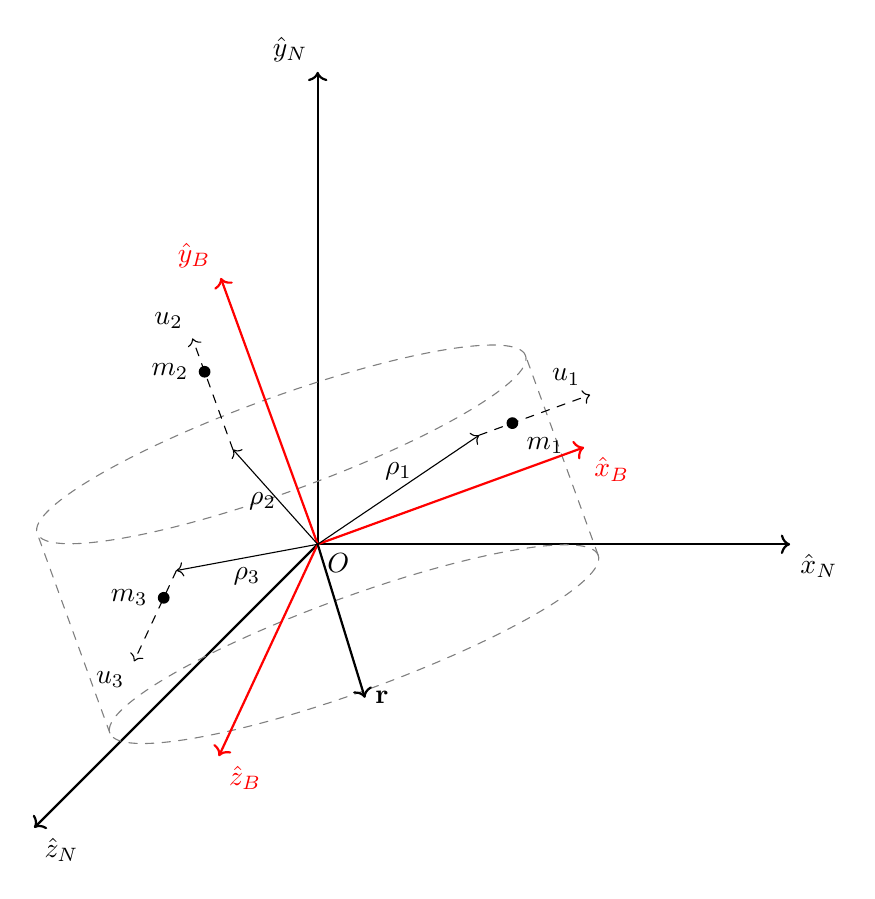
\begin{tikzpicture}[scale=3, line cap=round, line join=round]

% Inertial frame (I)
\draw[->, thick] (0,0) -- (2,0) node[below right] {$\hat{x}_N$};
\draw[->, thick] (0,0) -- (0,2) node[above left] {$\hat{y}_N$};
\draw[->, thick] (0,0) -- (-1.2,-1.2) node[below right] {$\hat{z}_N$};
\node[below right] at (0,0) {$O$};

% Cylinder representing platform ------------------------------
\pgfmathsetmacro{\radius}{1.1}
\pgfmathsetmacro{\height}{0.9}

\begin{scope}[rotate around={20:(0,0)}] 
    \draw[gray,dashed] (0,-\height/2) ellipse ({\radius} and 0.2);
    \draw[gray,dashed] (0,\height/2) ellipse ({\radius} and 0.2);
    \draw[gray,dashed] (-\radius,-\height/2) -- (-\radius,\height/2);
    \draw[gray,dashed] (\radius,-\height/2) -- (\radius,\height/2);
\end{scope} 

% Body frame (B), shifted and rotated
\begin{scope}[rotate=20]
    \draw[->, thick, red] (0,0) -- (1.2,0) node[below right] {$\hat{x}_B$};
    \draw[->, thick, red] (0,0) -- (0,1.2) node[above left] {$\hat{y}_B$};
    \draw[->, thick, red] (0,0) -- (-0.7,-0.7) node[below right] {$\hat{z}_B$};
    % \node[below left, red] at (0,0) {$\mathcal{B}$};

    % START M2 --------------------------------------
    \draw[->] (0,0) -- (-0.2,0.5) coordinate (rho2_end) 
        node[pos=0.65, below] {$\rho_2$};

    \draw[->, dashed] (rho2_end) -- ++(0,0.5) coordinate (u2_end)  
        node[above left] {$u_2$};

    \path (rho2_end) -- (u2_end) 
        node[pos=0.7, circle, fill=black, inner sep=1.5pt, label=left:$m_2$] {};

    % START M1 --------------------------------------
     \draw[->] (0,0) -- (0.8,0.2) coordinate (rho1_end) 
        node[midway, above] {$\rho_1$};

    \draw[->, dashed] (rho1_end) -- ++(0.5,0) coordinate (u1_end)  
        node[above left] {$u_1$};

    \path (rho1_end) -- (u1_end) 
        node[pos=0.3, circle, fill=black, inner sep=1.5pt, label=below right:$m_1$] {};

    % START M3 -----------------------------------
    \draw[->] (0,0) -- (-0.6,0.1) coordinate (rho3_end) 
        node[midway, below] {$\rho_3$};

    \draw[->, dashed] (rho3_end) -- ++(-0.3,-0.3) coordinate (u3_end)  
        node[below left] {$u_3$};

    \path (rho3_end) -- (u3_end) 
        node[pos=0.3, circle, fill=black, inner sep=1.5pt, label=left:$m_3$] {};
\end{scope}

% START COM r ----------------------------------
\draw[->, thick] (0,0) -- (0.2, -0.65) coordinate (r_end)
    node[below, right] {$\mathbf{r}$};
 




\end{tikzpicture}
    \caption{The mass balancing problem for air bearing based spacecraft dynamics simulators}
    \label{fig:tikz_venn}
\end{figure}


There are a variety of ways to measure and quantify this behavior. Assuming the center of mass is below the center of rotation, a very rough estimate for the torque due to gravity may be obtained by tilting the simulator about one of it's principal axes, releasing it, and observing the period of resulting pendulum motion $T$ \cite{kim_automatic_2009}. Let $\bm{r}$ denote the location of the center of mass with respect to the center of rotation. The torque is given by solving the below equation for $mg||\bm{r}||$
\begin{equation}
    T = 2\pi\sqrt{\frac{J_i}{mg||\bm{r}||}}
\end{equation}
where $J_i$ is the moment of inertia about said principle axis, $g$ is the acceleration due to gravity and $m$ is the overall mass of the simulator.

Another rough estimation method may be obtained by observing the total mechanical energy of the simulator while it undergoes pendulum said motion 
\begin{equation}
    E_{mech} = \frac{1}{2}\bm{\omega}^T\bm{J}\bm{\omega} + mgh
\end{equation}
where $\bm{\omega}$ is the angular velocity of the simulator, $\bm{J}$ is the inertia, and $h$ is the vertical height of $\bm{r}$ \cite{silva_filtering_2018}. If the simulator is balanced, $h$ will remain relatively constant throughout the pendulum motion, and the kinetic energy term $\frac{1}{2}\bm{\omega}^T\bm{J}\bm{\omega}$ will also remain relatively constant due to the conservation of energy. As the balance of the simulator improves, the kinetic energy will oscillate with smaller amplitudes.

Ideally this value is zero, but in practice mass balancing systems seek to make this value as small as possible while satsifying other project constraints like cost, time, and volume. 


\section{Mass Balancing Hardware}

\section{Batch Estimation Algorithms}

\section{Kalman Filtering for Inbalance Estimation}

\section{Active Control for Balancing}

\section{Cal Poly SADS MBS Design }
\begin{table}[h!]
\caption{Existing spacecraft dynamics simulators and their balancing methods}\label{table:existing_testbeds}
\centering
\renewcommand{\arraystretch}{1.3}

\begin{tabularx}{\textwidth}{
    >{\raggedright\arraybackslash}p{3cm}   % Institution
    >{\raggedright\arraybackslash}p{3.5cm} % Actuators
    >{\raggedright\arraybackslash}p{2.2cm} % Noise Density
    >{\raggedright\arraybackslash}X}       % Balancing Method and Results
\toprule
\textbf{Institution} & \textbf{Actuators} & \textbf{Noise Density} & \textbf{Balancing Method and Results} \\
\midrule
Cal Poly San Luis Obispo~\cite{dam_applied_2014} & 
Reaction Wheels & 
\SI{0.0025}{\degree\per\second} & 
Batch Estimation \newline $<\SI{1.5}{\milli\metre}$ \\
\addlinespace[0.75em]

Georgia Tech~\cite{choi_automatic_2016} & 
Reaction Wheels & 
\SI{0.05}{\degree\per\second} & 
Underactuated Feedback Control \\
\addlinespace[0.75em]
Naval Postgraduate School~\cite{kim_system_2006} & 
Control Moment Gyros & 
\SI{0.007}{\degree\per\second} & 
Fully Actuated Feedback Control \newline $<\SI{0.327}{\newton\metre}$ \\
\addlinespace[0.75em]
University of Brasília~\cite{silva_filtering_2018} & 
Reaction Wheels, Magnetorquers & 
\SI{0.05}{\degree\per\second} & 
Batch Estimation and Filtering \newline $<\num{3.5e-5}\,\si{\newton\metre}$ \\
\addlinespace[0.75em]
University of Bologna~\cite{modenini2020dynamic} & 
Reaction Wheels & 
\SI{0.004}{\degree\per\second} & 
Underactuated Feedback Control \newline $<\num{5e-5}\,\si{\newton\metre}$ \\
\addlinespace[0.75em]
University of Florida~\cite{saulnier2014six} & 
Thrusters & 
N/A & 
Manual Balancing \\
\addlinespace[0.75em]
Harbin Institute of Technology~\cite{xu_parameter_2015} & 
Reaction Wheels & 
\SI{0.04}{\degree\per\second} & 
Batch Estimation and Filtering \newline $<\SI{5}{\micro\metre}$ \\
\bottomrule
\end{tabularx}

\vspace{0.5em}
\raggedright\footnotesize
\textit{Note: Balancing results are included as reported. Results are either listed as the maximum torque due to gravity measured during testing or the estimated center of mass offset.}
\end{table}
